%----------------------------------------------------------------------------------------
%	PACKAGES AND THEMES
%----------------------------------------------------------------------------------------
\documentclass[aspectratio=43,xcolor=dvipsnames]{beamer}
\usetheme{SimplePlus}
\usepackage[utf8]{vietnam}
\usepackage{subfigure}
\usepackage{hyperref}
\usepackage{graphicx}
\usepackage{booktabs} 
\usepackage{amsmath}
%----------------------------------------------------------------------------------------
%	TITLE PAGE
%----------------------------------------------------------------------------------------
%[plain, noframenumbering]
\title[short title]{HUSTFood}
%\subtitle{\Large{Trang web đồ ăn cho sinh viên Bách Khoa}}

\institute[HUST]
{
	Trường Công nghệ Thông tin và Truyền thông \\
	Đại học Bách Khoa Hà Nội
}
\date{Ngày 25 tháng 7 năm 2022}


%----------------------------------------------------------------------------------------
%	PRESENTATION SLIDES
%----------------------------------------------------------------------------------------

\begin{document}
	
	\begin{frame}[plain, noframenumbering]
		\titlepage
	\end{frame}
	\begin{frame}[plain, noframenumbering]{Thành viên trong nhóm}
		\begin{table}[!h]
			% \centering
			\label{ba2}
			\scalebox{1.2}{
				\begin{tabular}{|c|c|} \hline
					\textbf{Họ tên} & \textbf{MSSV}  \\ \hline 
					Phan Minh Anh Tuấn  & 20205227\\ 
					Nguyễn Thị Hoài Linh & 20205231\\ 
					Vũ Minh Long & 20200373\\ 
					Đàm Ngọc Khánh & 20205207\\ \hline 
				\end{tabular}
			}
		\end{table}
		% \begin{itemize}
			%     \item Phan Minh Anh Tuấn - 20205227
			%     \item Nguyễn Thị Hoài Linh - 20205231
			%     \item Vũ Minh Long - 20200373
			%     \item Đàm Ngọc Khánh - 20205207
			% \end{itemize}
	\end{frame}
	\begin{frame}[plain, noframenumbering]{Các thành phần chính}
		\tableofcontents
	\end{frame}
	%------------------------------------------------
	\section{Giới thiệu}
	\begin{frame}{Giới thiệu}
    \begin{itemize}
        \item \large{\textbf{HUSTFood}} - Web đặt đồ ăn cho sinh viên Bách Khoa
	    \item Xây dựng cơ sở dữ liệu quản lý thông tin người dùng, nhà hàng (món ăn), đặt hàng (người dùng - đơn hàng - nhà hàng), chương trình khuyến mãi (nhà hàng - mã giảm giá)...
		\item \textbf{HUSTFood} cho phép người dùng:
	        \begin{itemize}
	            \item Tạo tài khoản, đăng nhập vào trang web
	            \item Bổ sung thông tin
	            \item Tìm kiếm nhà hàng, món ăn
	            \item Đặt hàng
	        \end{itemize}
    \end{itemize}
	

	\end{frame}
	%------------------------------------------------
	\section{Cơ sở dữ liệu}
	\begin{frame}{Tổng quan Database}
		\begin{figure}[ht!]
			\centerline{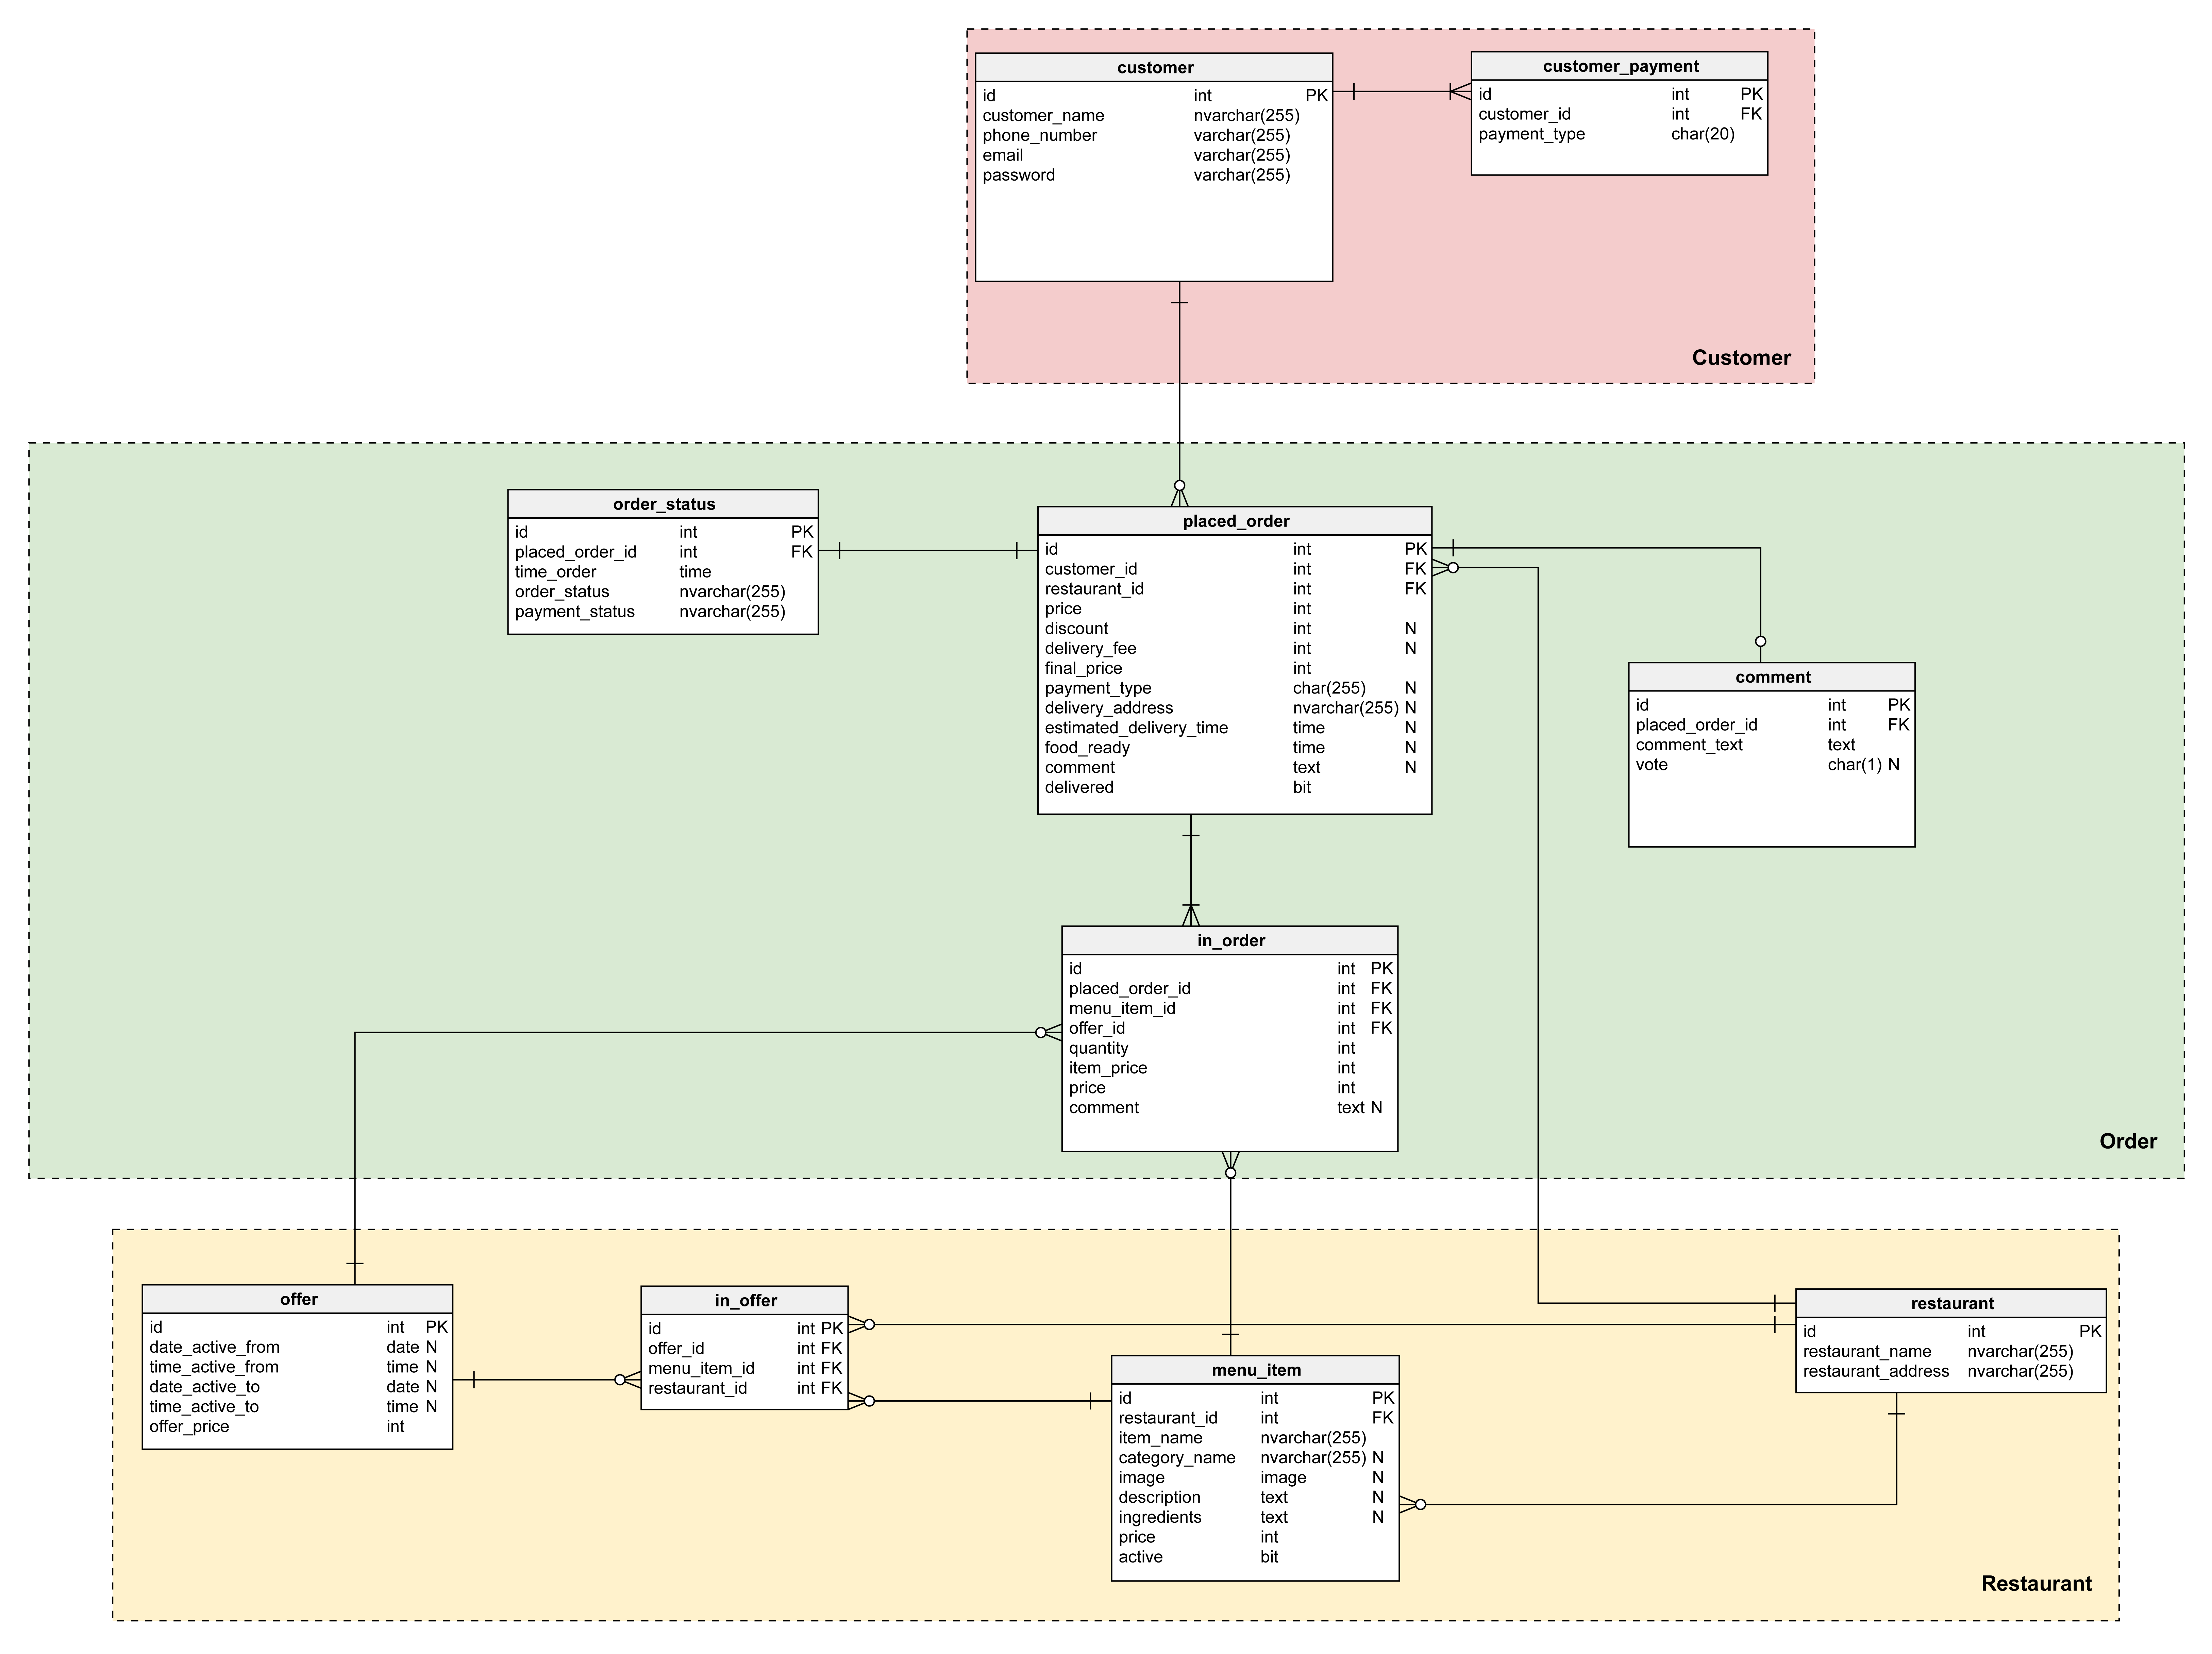
\includegraphics[width=0.9\textwidth]{sql_1.png}}
			\label{fig:ass1}
		\end{figure}
	\end{frame}
	\subsection{Customer}
	\begin{frame}[plain, noframenumbering]
		\textcolor{structure}{\Huge{\textbf{Customer}}}
	\end{frame}
	%------------------------------------------------
	\begin{frame}{Customer}
		\begin{figure}[ht!]
			\centerline{\includegraphics[width=1\textwidth]{customer.png}}
			\label{fig:ass1}
		\end{figure}
	\end{frame}
	\begin{frame}{Customer}
		\textcolor{structure}{\large{\textbf{Customer:}}}
		\begin{itemize}
			\item \textbf{id:} Primary key
			\item \textbf{customer$\_$name:} Tên khách hàng
			\item \textbf{phone$\_$number:} Số điện thoại khách hàng
			\item \textbf{email:} Email khách hàng (Unique)
			\item \textbf{password:} Mật khẩu tài khoản
		\end{itemize}
		\pause
		\textcolor{structure}{\large{\textbf{Customer\_payment}}}
		\begin{itemize}
			\item \textbf{id:} Primary key
			\item \textbf{customer\_id:} Foreign key customer(id)
			\item \textbf{payment\_type:} Phương thức thanh toán (Momo/Zalopay/VTMoney/ShopeePay/Cash)
		\end{itemize}
	\end{frame}
	\begin{frame}{Customer}
		\begin{figure}[ht!]
			\centerline{\includegraphics[width=1\textwidth]{customer.png}}
			\label{fig:ass1}
		\end{figure}
	\end{frame}
	\subsection{Order}
	\begin{frame}[plain, noframenumbering]
		\textcolor{structure}{\Huge{\textbf{Order}}}
	\end{frame}
	\begin{frame}{Order}
		\begin{figure}[ht!]
			\centerline{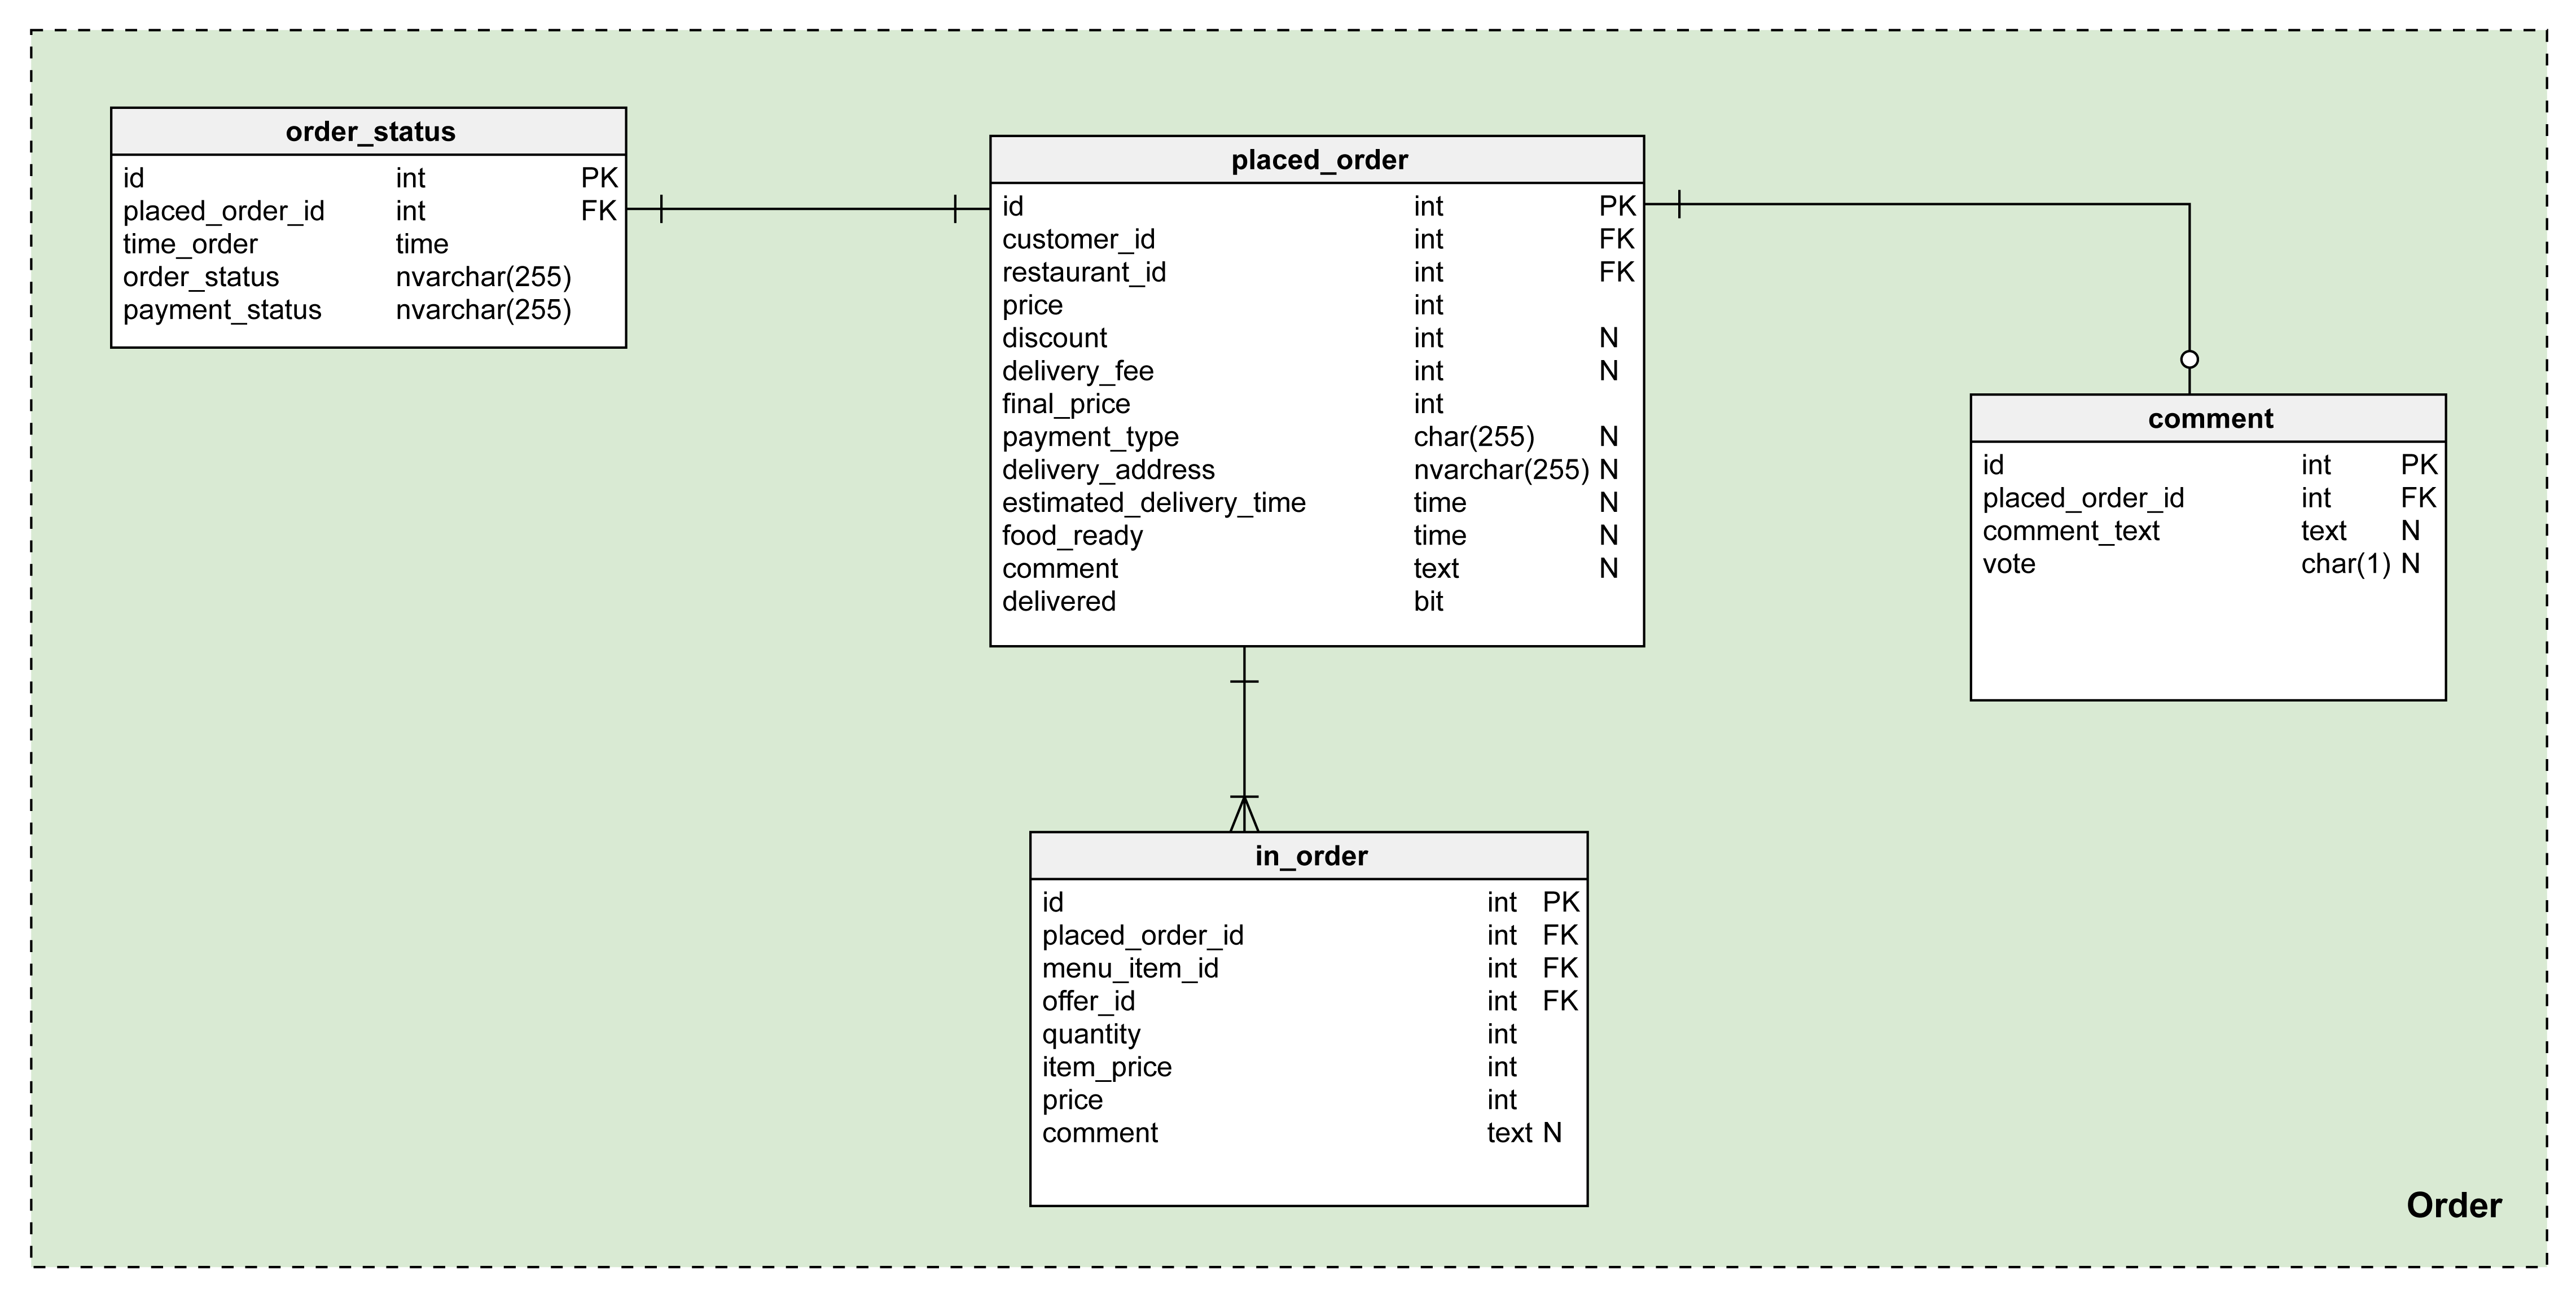
\includegraphics[width=1\textwidth]{order.png}}
			\label{fig:ass1}
		\end{figure}
	\end{frame}
	\begin{frame}{Placed Order}
		\begin{itemize}
			\item \textbf{id:} Primary key
			\item \textbf{customer\_id:} Foreign key customer(id)
			\item \textbf{restaurant\_id:} Foreign key restaurant(id)
			\item \textbf{price:} Giá ban đầu
			\item \textbf{discount:} Giảm giá 
			\item \textbf{delivery\_fee: }Phí vận chuyển
			\item \textbf{final\_price:} Giá phải trả
			\item \textbf{payment\_type:} Hình thức thanh toán
			\item \textbf{delivery\_address:} Địa chỉ giao hàng 
			\item \textbf{estimated\_delivery\_time:} Thời gian dự kiến giao hàng
			\item \textbf{food\_ready:} Đồ ăn đã sẵn sàng chưa
			\item \textbf{comment:} Lưu ý của khách hàng
			\item \textbf{deliveried:} Đã được giao hay chưa
		\end{itemize}
	\end{frame}
	
	\begin{frame}{Order status}
		\begin{itemize}
			\item \textbf{id:} Primary key
			\item \textbf{placed\_order\_id:} Foreign key placed\_order(id)
			\item \textbf{time\_order:} Thời gian đặt hàng
			\item \textbf{order\_status:} Trạng thái đơn hàng (Thêm vào giỏ / Xác nhận / Đã thanh toán / Đã giao)
			\item \textbf{payment\_status:} Trạng thái thanh toán (Chưa xác nhận / Đã xác nhận)
		\end{itemize}
	\end{frame}
	
	\begin{frame}{In order}
		\begin{itemize}
			\item \textbf{id:} Primary key
			\item \textbf{placed\_order\_id:} Foreign key placed\_order(id)
			\item \textbf{offer\_id:} Foreign key offer(id)
			\item \textbf{menu\_item\_id:} Foreign key menu\_item(id)
			\item \textbf{quantity:} Số lượng mua
			\item \textbf{item\_price:} Đơn giá
			\item \textbf{price:} Tổng số tiền phải trả
			\item \textbf{comment:} Lưu ý của khách hàng
		\end{itemize}
	\end{frame}
	
	\begin{frame}{Comment}
		\begin{itemize}
			\item \textbf{id:} Primary key
			\item \textbf{placed\_order\_id:} Foreign key placed\_order(id)
			\item \textbf{customer\_id:} Foreign key customer(id)
			\item \textbf{comment\_text:} Đánh giá của khách hàng
			\item \textbf{vote:} Đánh giá trên thang 5 sao, nhận giá trị null nếu khách hàng không đánh giá
		\end{itemize}
	\end{frame}
	\begin{frame}{Order}
		\begin{figure}[ht!]
			\centerline{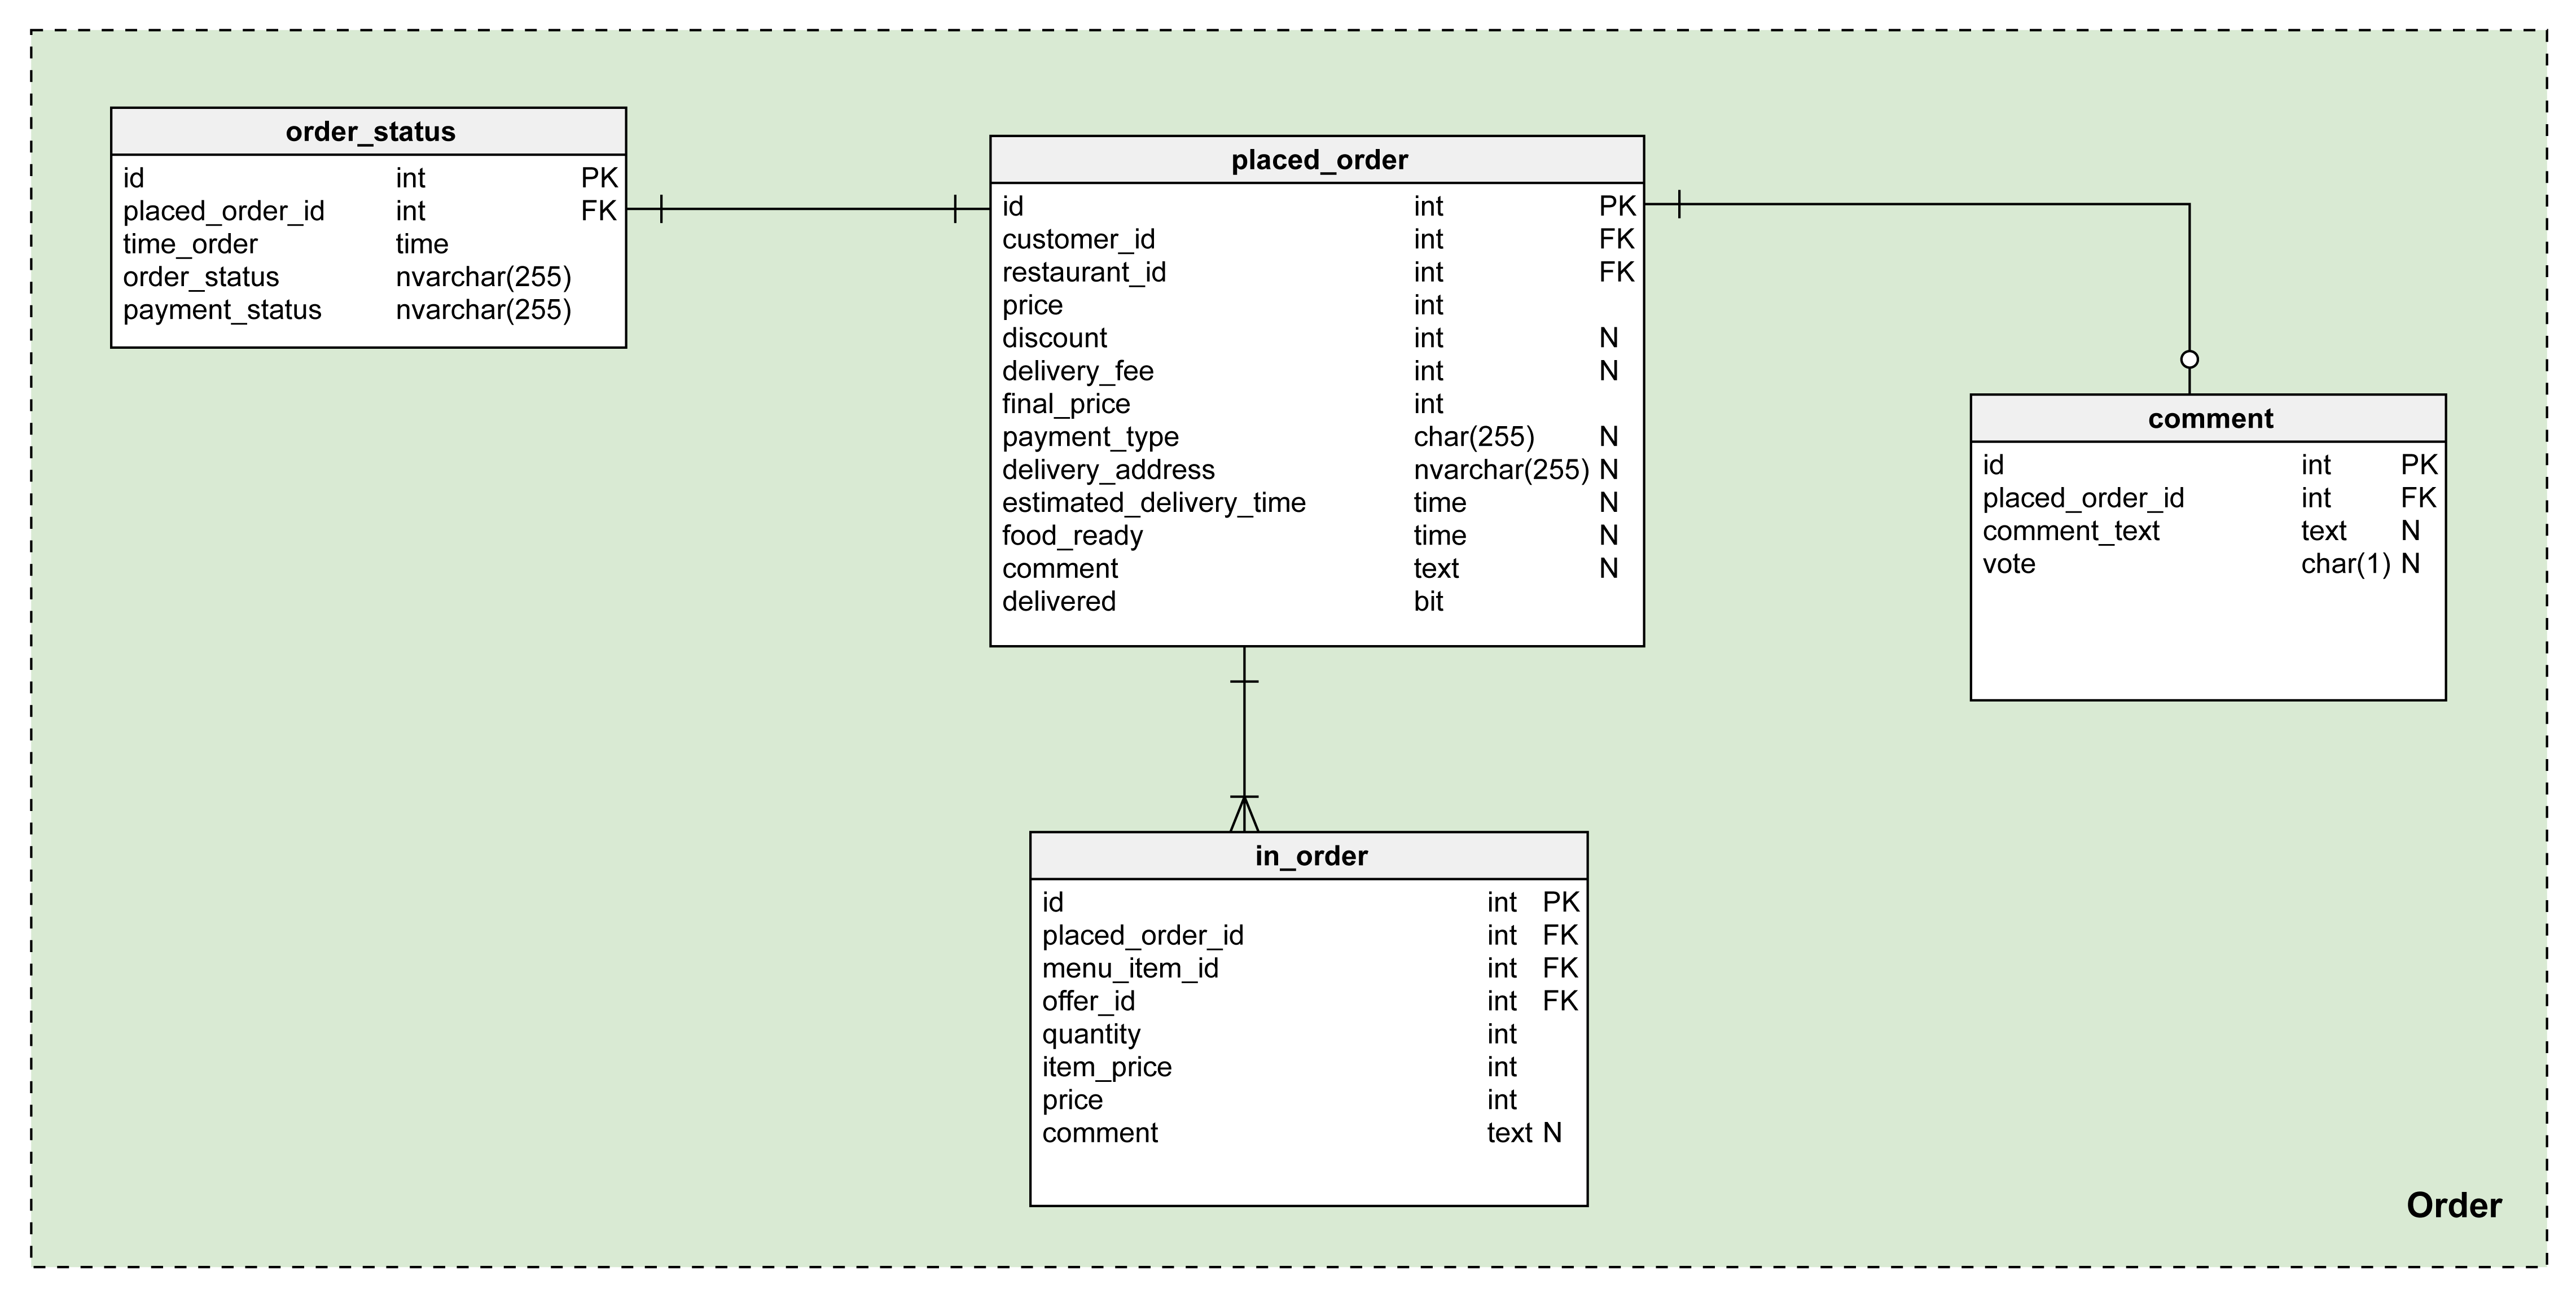
\includegraphics[width=1\textwidth]{order.png}}
			\label{fig:ass1}
		\end{figure}
	\end{frame}
	\subsection{Restaurant}
	\begin{frame}[plain, noframenumbering]
		\textcolor{structure}{\Huge{\textbf{Restaurant}}}
	\end{frame}
	\begin{frame}{Restaurant}
		\begin{figure}[ht!]
			\centerline{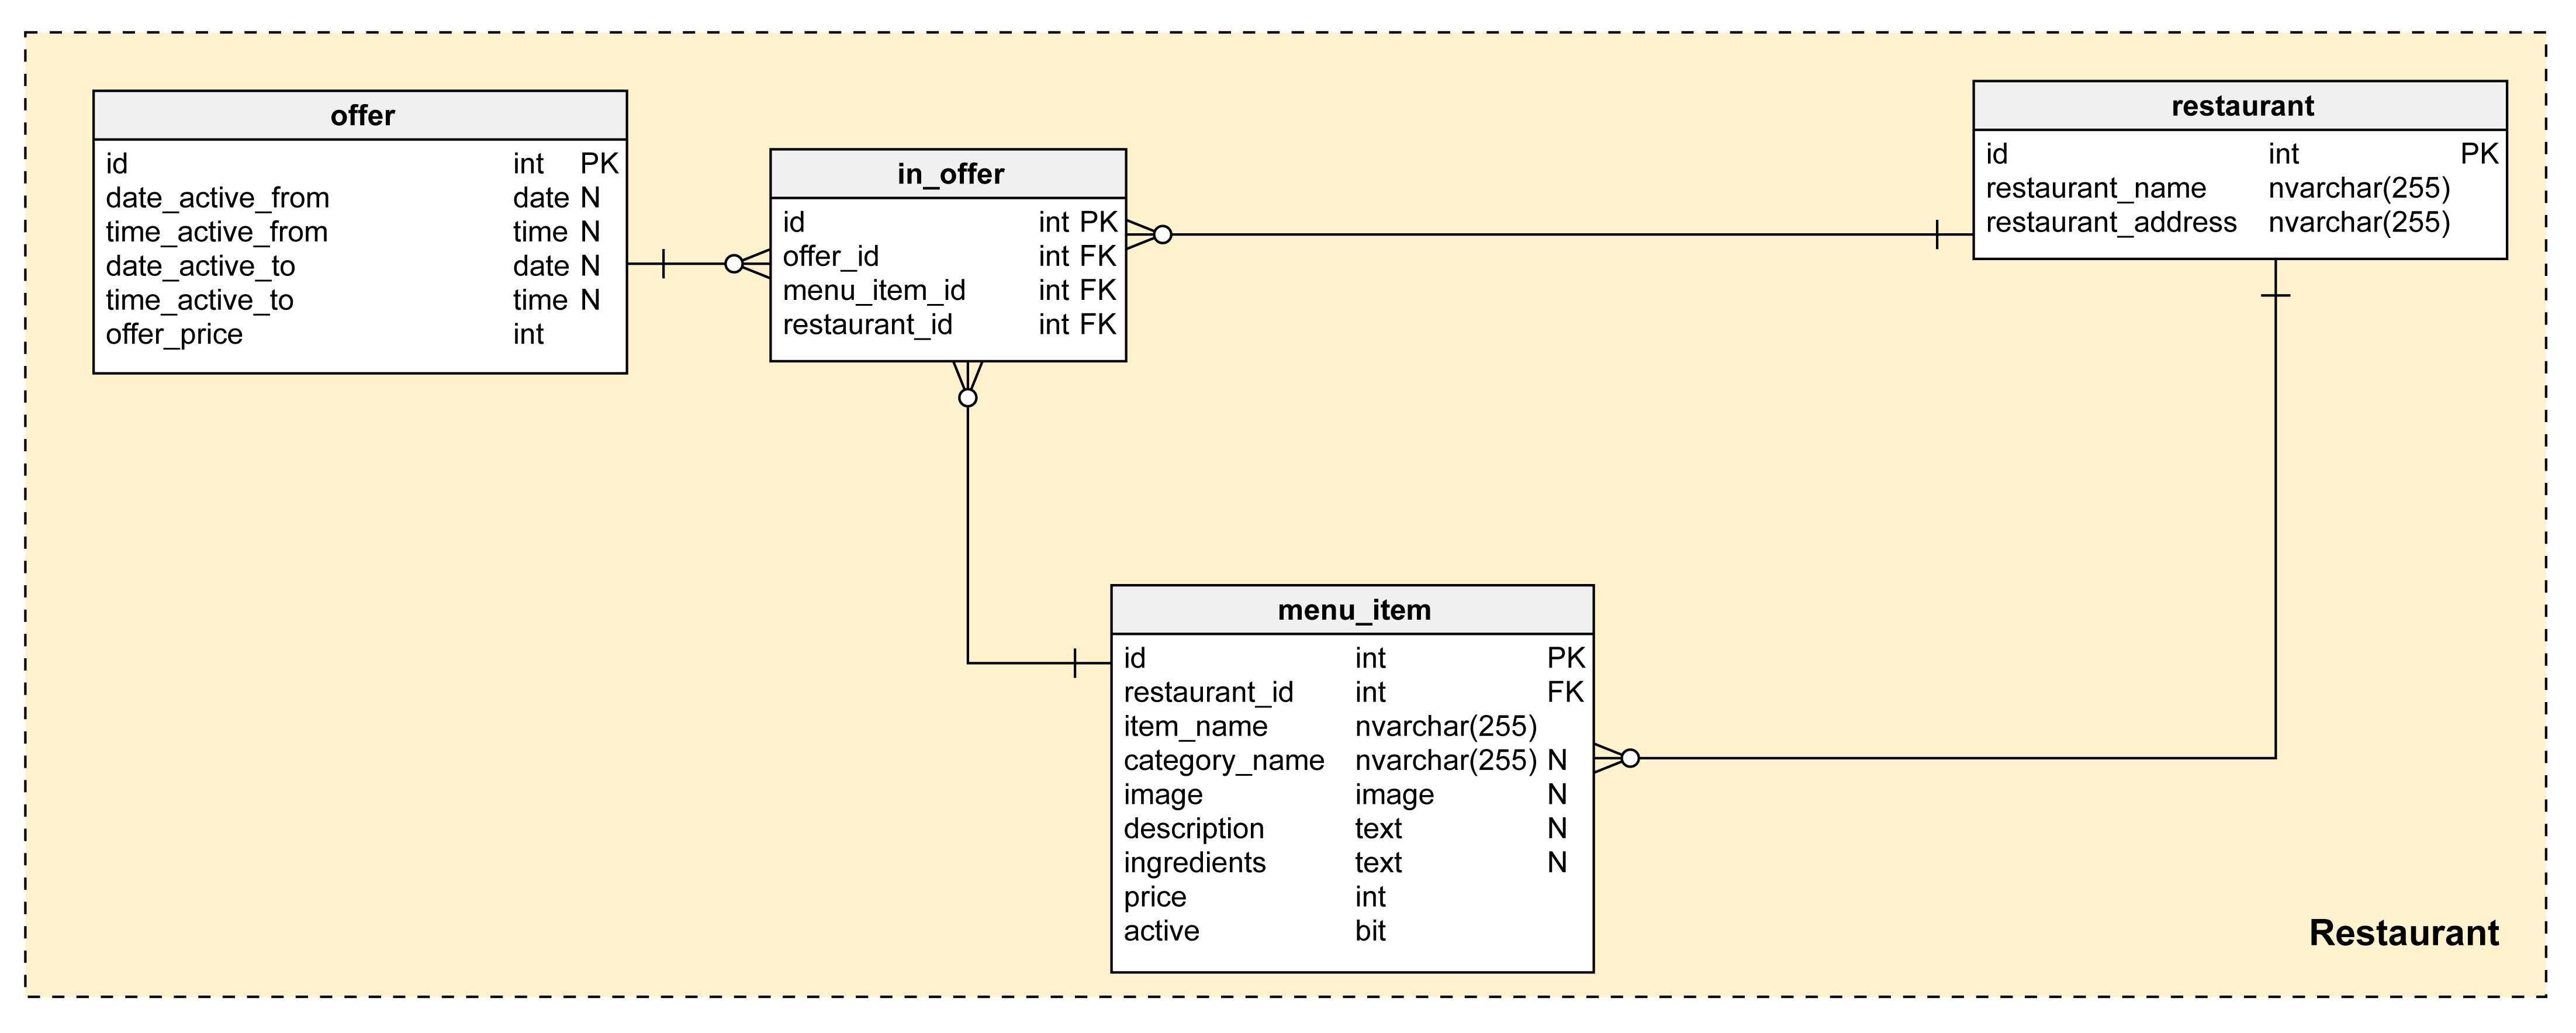
\includegraphics[width=1\textwidth]{restaurant.png}}
			\label{fig:ass1}
		\end{figure}
	\end{frame}
	\begin{frame}{Menu item}
		\begin{itemize}
			\item \textbf{id:} Primary key
			\item \textbf{restaurant\_id:} Foreign key restaurant(id)
			\item \textbf{item\_name:} Tên món ăn
			\item \textbf{category\_name:} Phân loại
			\item \textbf{image:} Hình ảnh
			\item \textbf{description:} Mô tả
			\item \textbf{ingredients:} Nguyên liệu
			\item \textbf{price:} Đơn giá
			\item \textbf{active:} Tình trạng mặt hàng (còn hay hết)
		\end{itemize}
	\end{frame}
	
	\begin{frame}{Restaurant}
		\begin{itemize}
			\item \textbf{id:} Primary key
			\item \textbf{restaurant\_name:} Tên nhà hàng
			\item \textbf{restaurant\_address:} Địa chỉ
		\end{itemize}
	\end{frame}
	
	\begin{frame}{Offer}
		\begin{itemize}
			\item \textbf{id:} Primary key
			\item \textbf{data\_active\_from:} Ngày bắt đầu kích hoạt
			\item \textbf{time\_active\_from:} Giờ bắt đầu kích hoạt
			\item \textbf{data\_active\_to:} Ngày kết thúc kích hoạt
			\item \textbf{time\_active\_to:} Giờ kết thúc kích hoạt
			\item \textbf{offer\_price:} Giá trị ưu đãi
		\end{itemize}
	\end{frame}
	\begin{frame}{In offer}
		%Lưu thông tin giảm giá với mặt hàng tương ứng (sale thì mỗi mặt hàng 1 kiểu)
		\begin{itemize}
			\item \textbf{id:} Primary key
			\item \textbf{offer\_id: } Foreign key offer(id)
			\item \textbf{menu\_item\_id: } Foreign key menu\_item(id)
			\item \textbf{restaurant\_id: } Foreign key restaurant(id)
		\end{itemize}
	\end{frame}

	\begin{frame}{Restaurant}
		\begin{figure}[ht!]
			\centerline{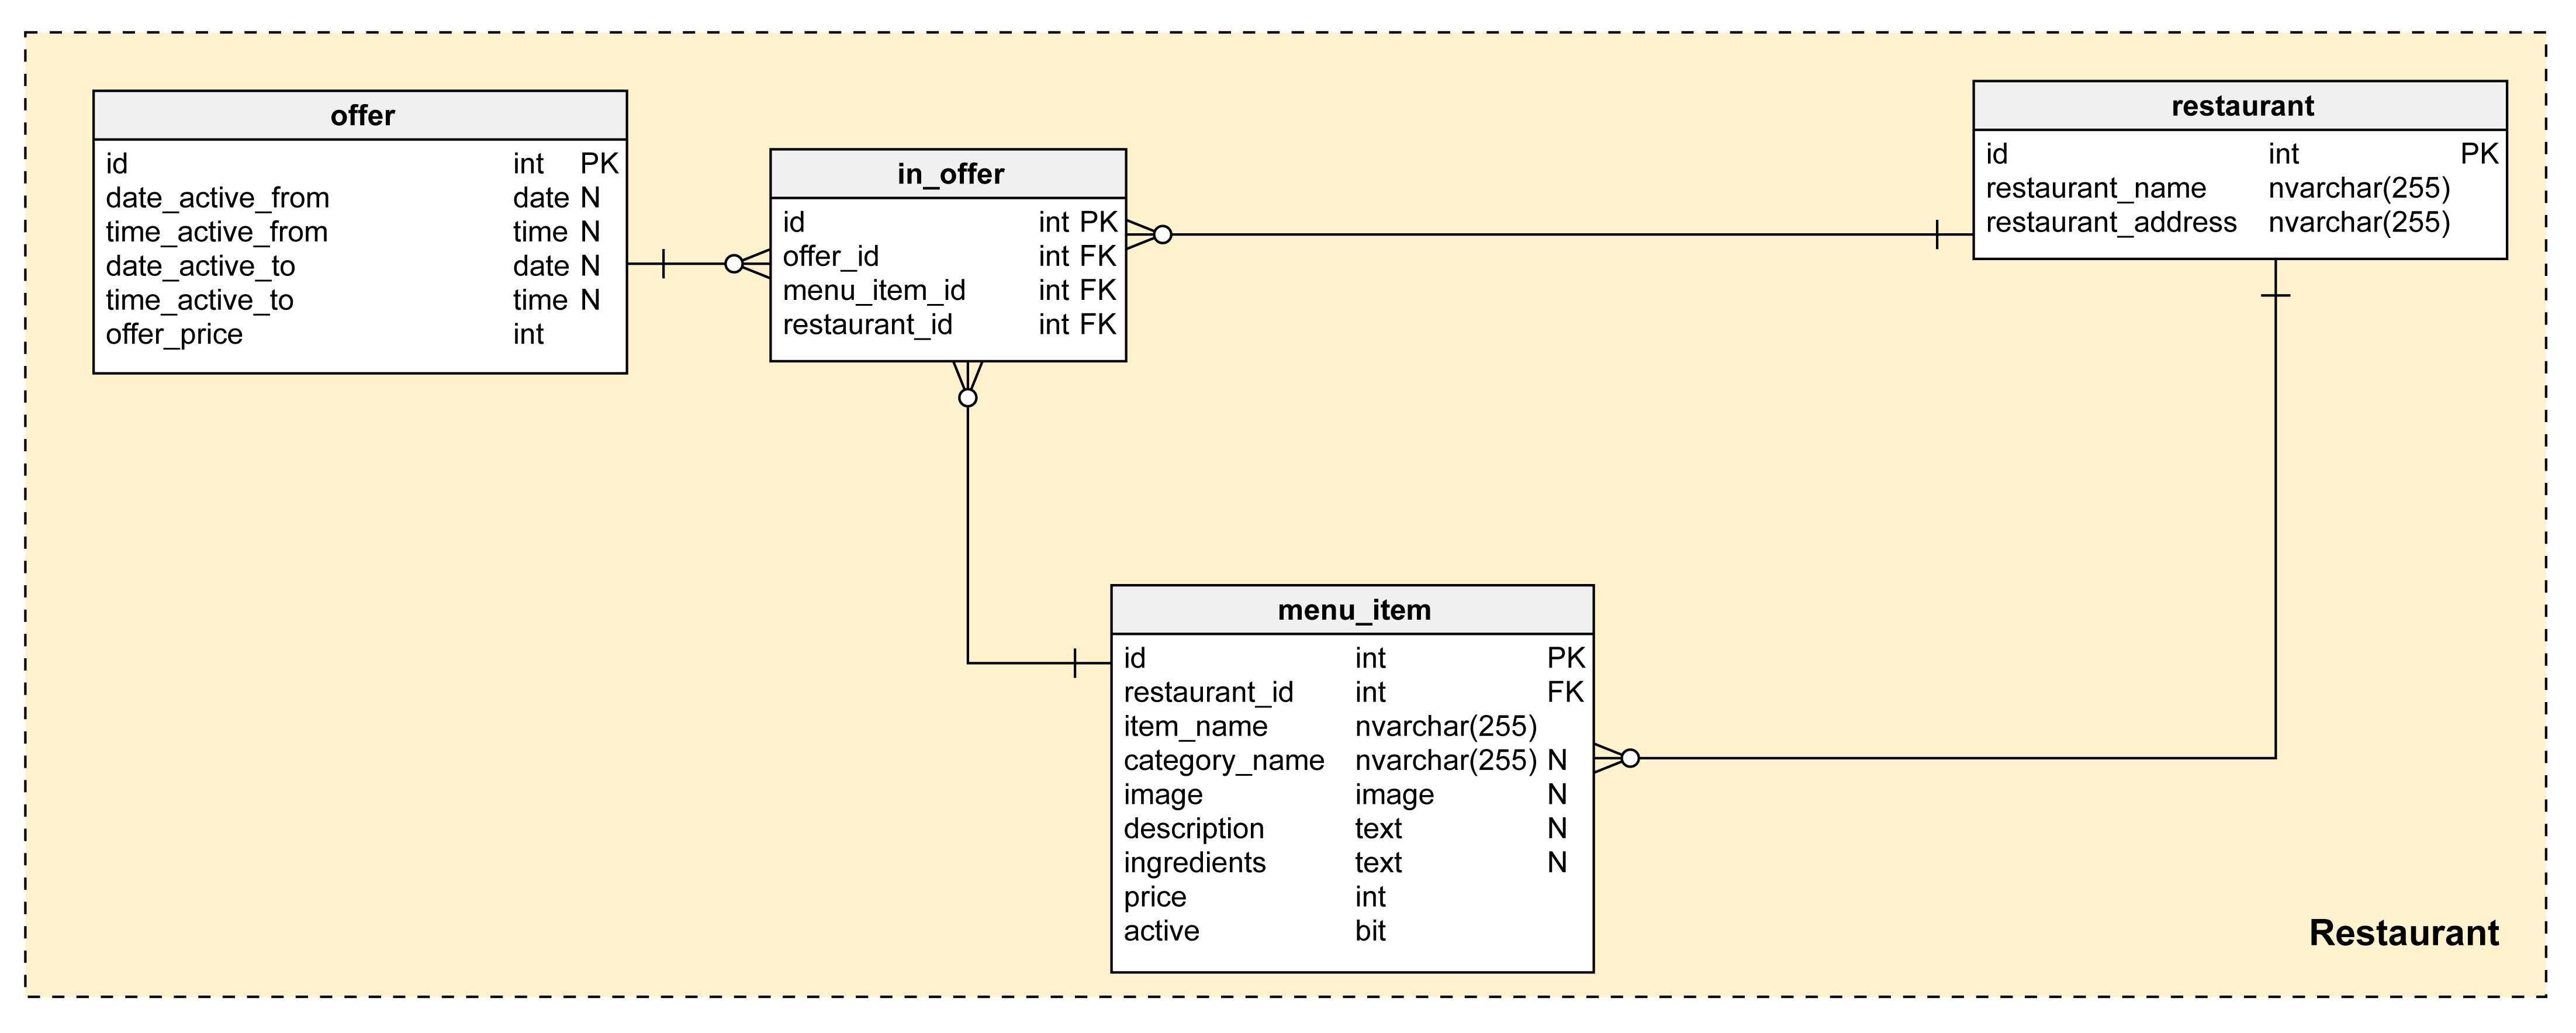
\includegraphics[width=1\textwidth]{restaurant.png}}
			\label{fig:ass1}
		\end{figure}
	\end{frame}
	
	%----------------------------------------------------------------------------------------
	\section{Sản phẩm}
	\begin{frame}[plain, noframenumbering]
		\textcolor{structure}{\Huge{\textbf{Sản phẩm}}}
	\end{frame}
	\subsection{Tổng quan}
	\begin{frame}{Tổng quan}
	\textcolor{structure}{\large{\textbf{Các thư viện cần dùng}}}
		\begin{itemize}
			\item \textbf{Python Flask:} Xây dựng backend của trang web 
			\item \textbf{Pyodbc:} Kết nối web đến SQL Server Database
		\end{itemize}
    \end{frame}
	\subsection{Trang chủ}
	\begin{frame}{Trang chủ}
	Cho phép người dùng đăng ký tài khoản, đăng nhập và tìm kiếm nhà hàng, món ăn (kể cả khi không đăng nhập).		
	\begin{figure}[ht!]
		\centerline{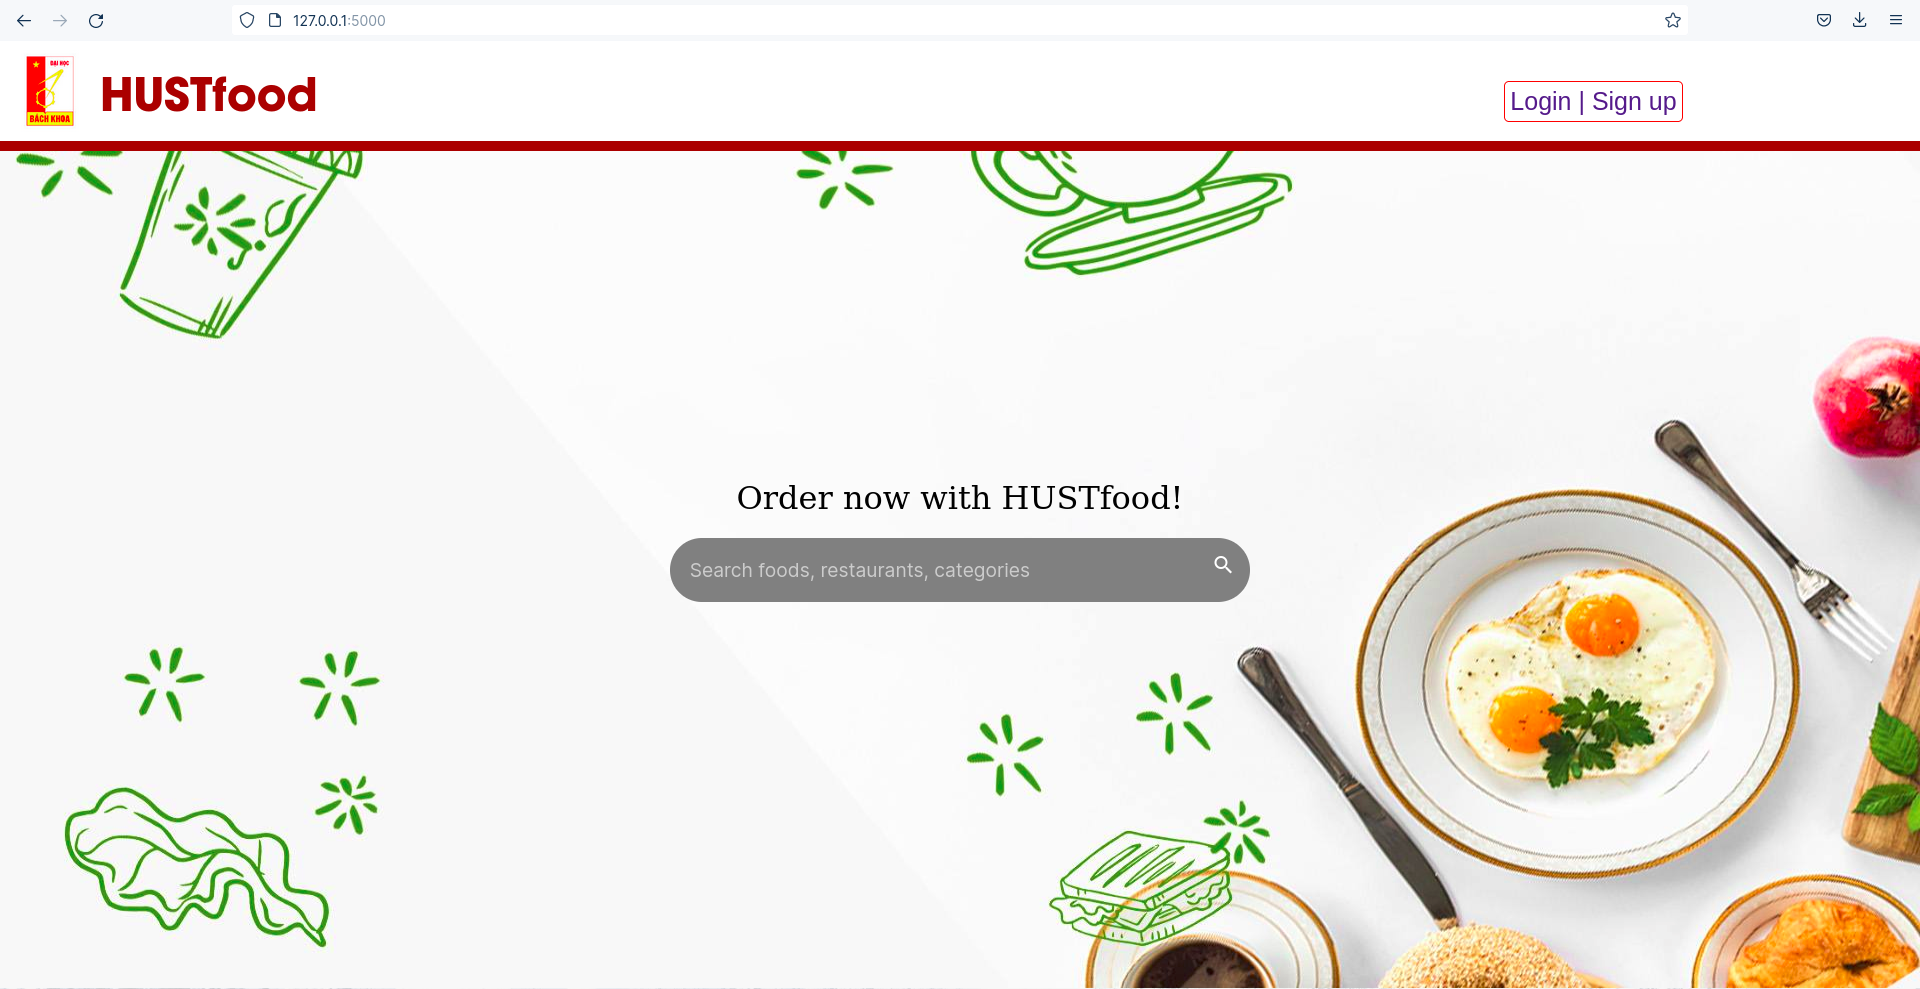
\includegraphics[width=0.9\textwidth]{web-image/trangchu_chuadn.png}}
		\caption{Giao diện trang chủ web}
		\label{fig:ass1}
	\end{figure}
	\end{frame}
	\subsection{Đăng ký}
	\begin{frame}{Đăng ký}
	Cho phép người dùng đăng ký tài khoản mới với thông tin xác định là Email (mỗi Email chỉ có thể đăng ký một tài khoản duy nhất).
		\begin{figure}[ht!]
			\centerline{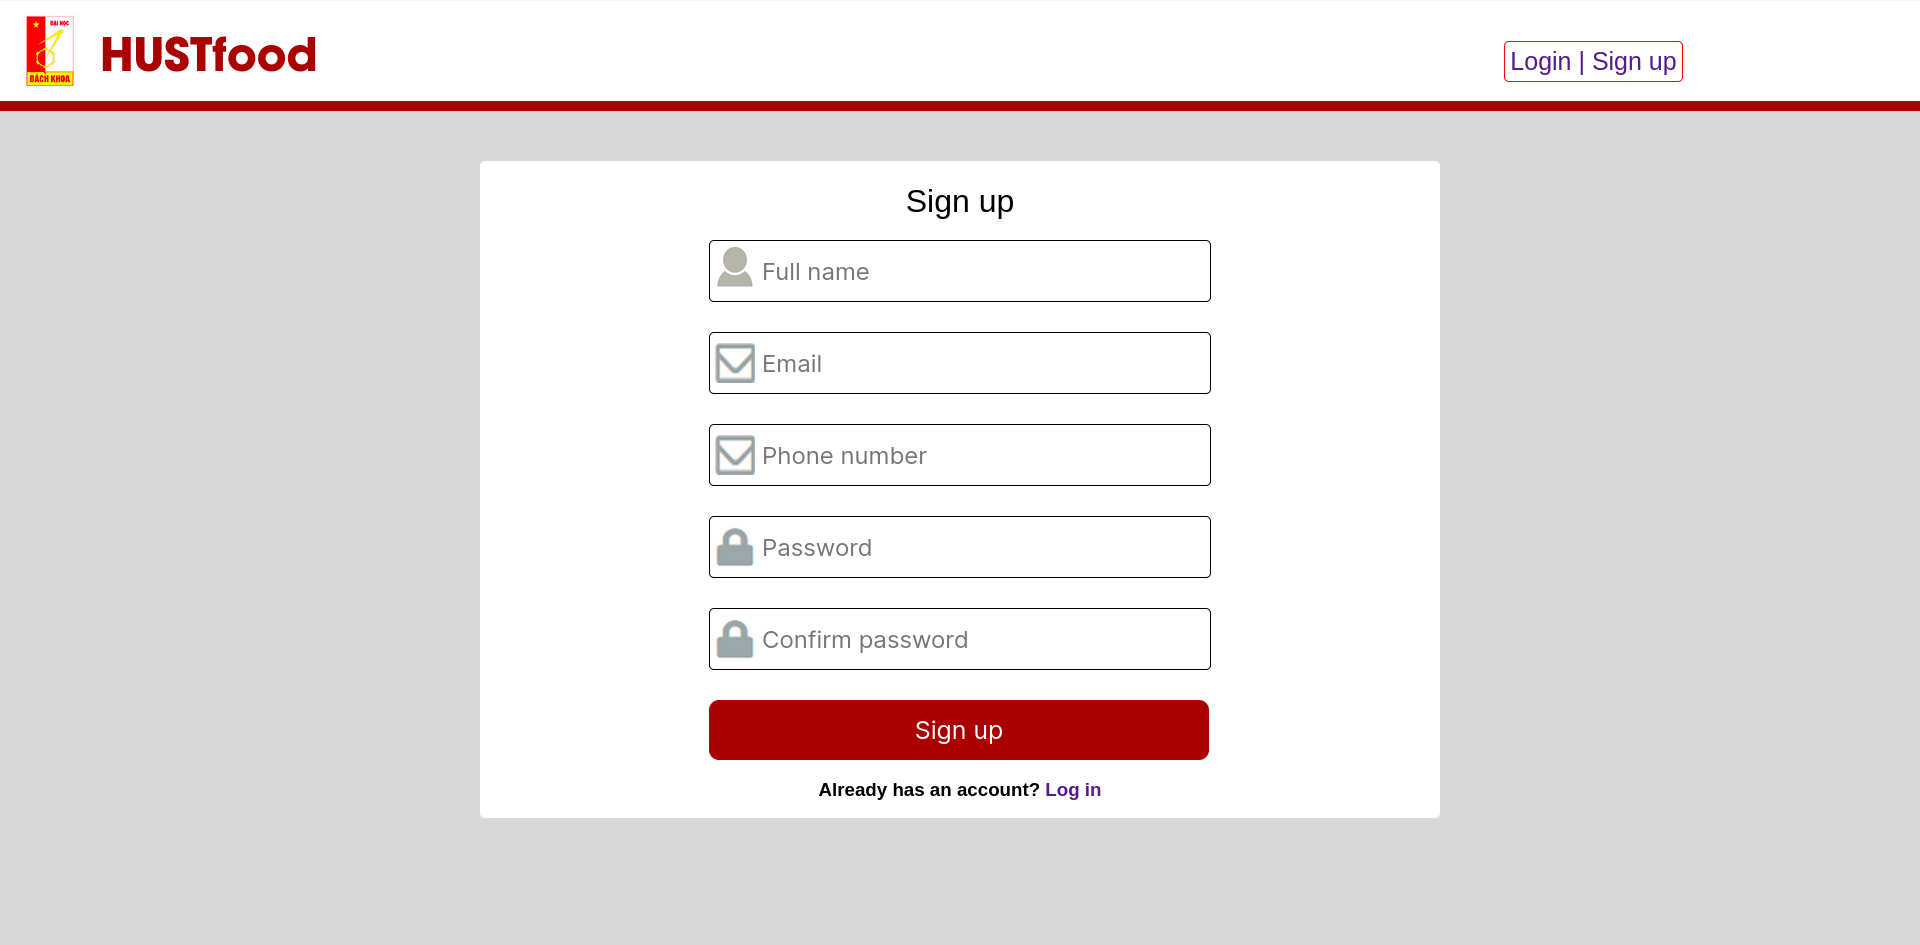
\includegraphics[width=0.9\textwidth]{web-image/dangky.png}}
			\caption{Giao diện đăng ký thông tin người dùng}
			\label{fig:ass1}
		\end{figure}
	\end{frame}
	\subsection{Đăng nhập}
	\begin{frame}{Đăng nhập}
	Yêu cầu người dùng nhập email và mật khẩu để đăng nhập vào tài khoản.
		\begin{figure}[ht!]
			\centerline{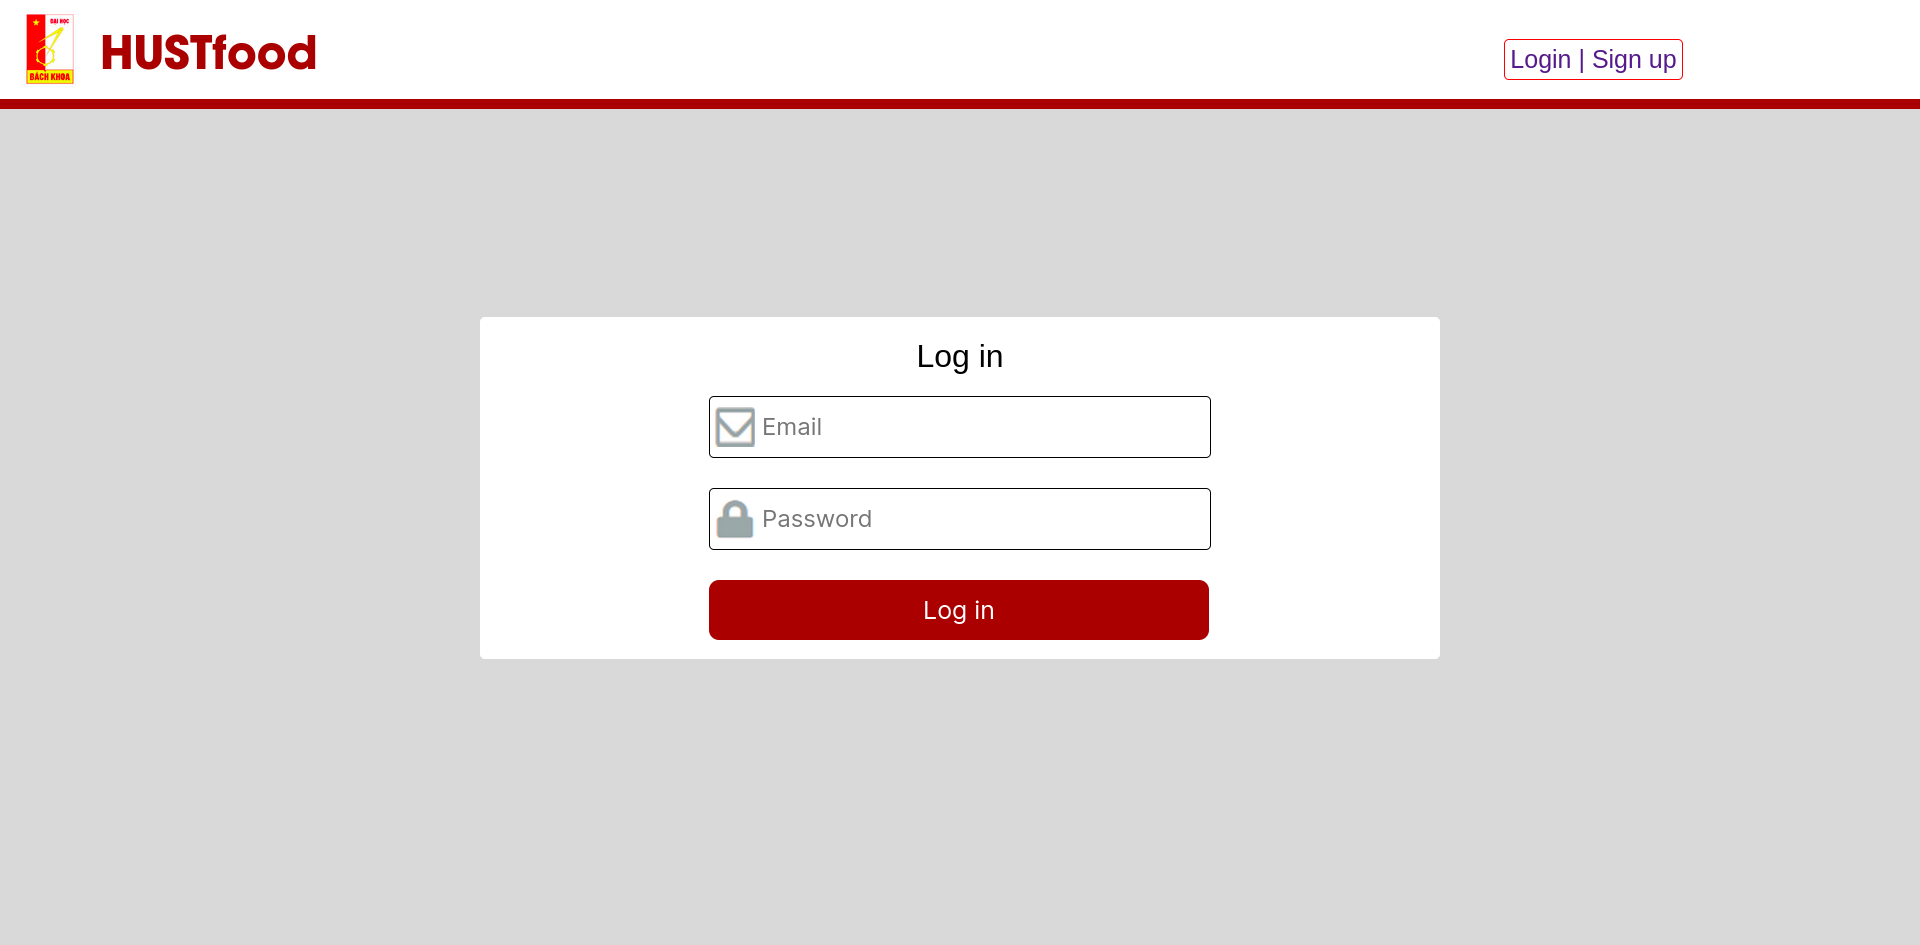
\includegraphics[width=0.9\textwidth]{web-image/dangnhap.png}}
			\caption{Giao diện đăng nhập}
			\label{fig:ass1}
		\end{figure}
	\end{frame}
	\subsection{Thông tin người dùng}
	\begin{frame}{Thông tin người dùng}
	Xuất hiện khi click vào avatar người dùng, cho biết thông tin của người dùng (tên, số điện thoại, email, phương thức thanh toán) và cho phép xem, chỉnh sửa phương thức thanh toán.
		\begin{figure}[ht!]
			\centerline{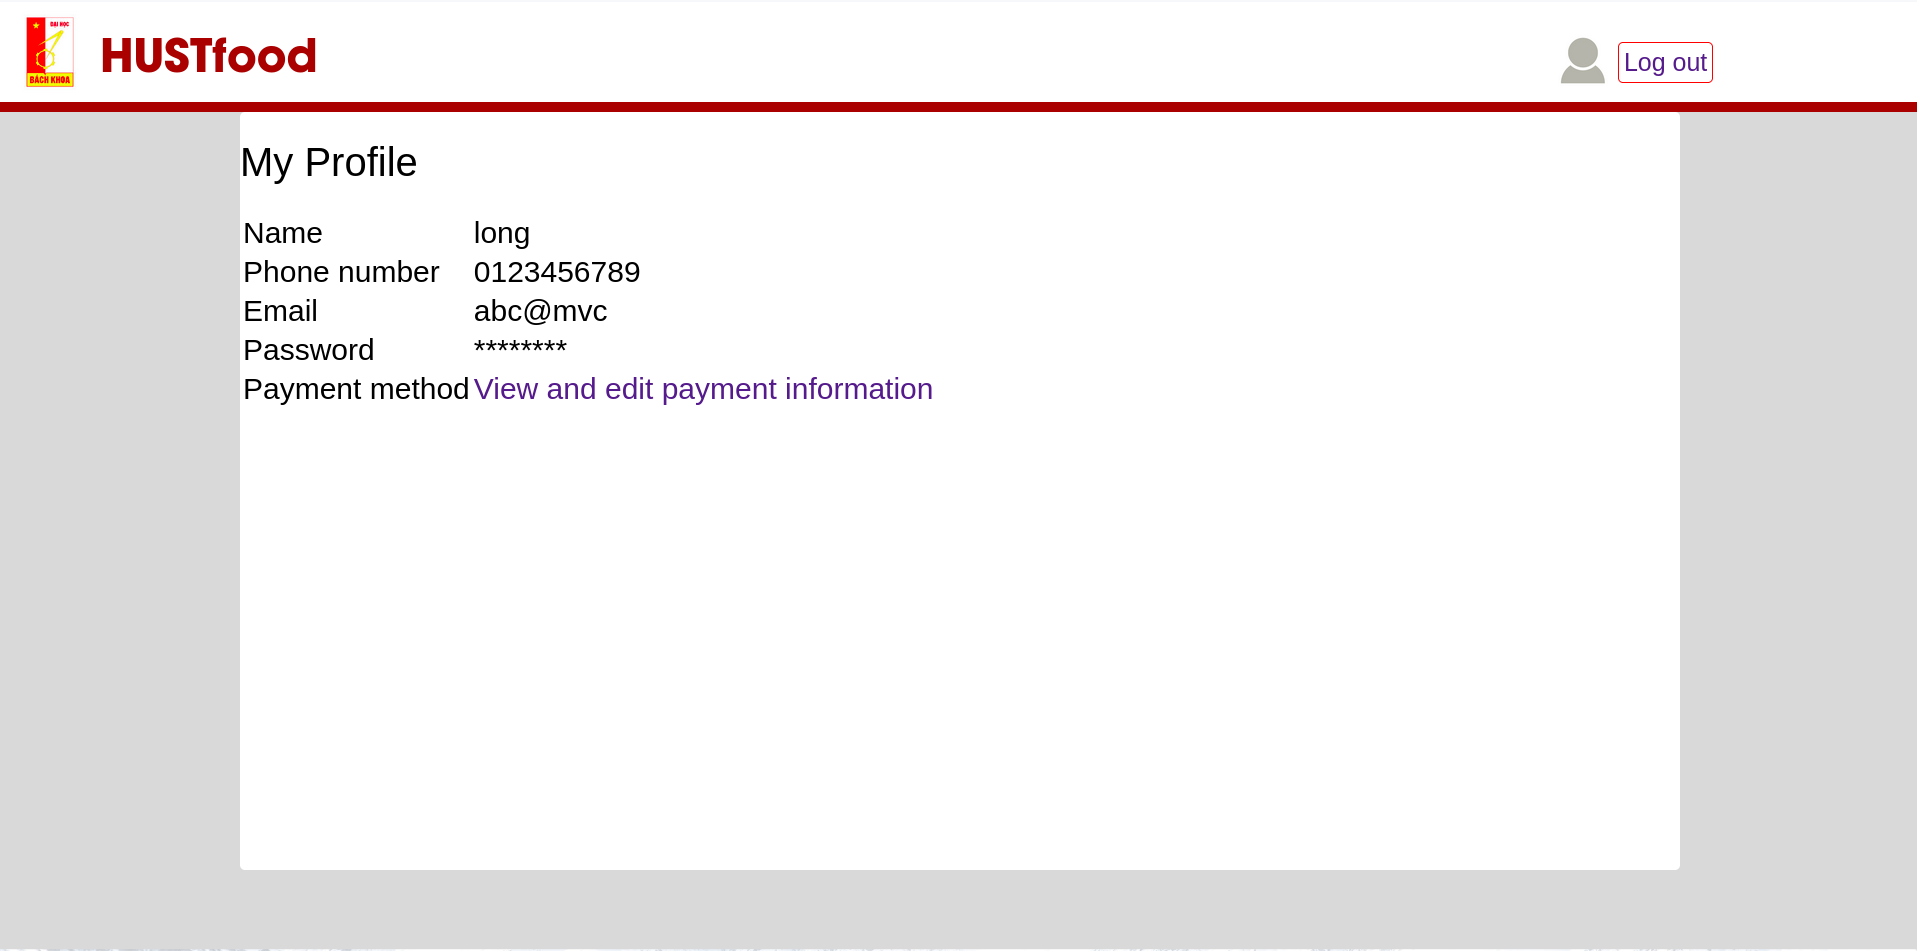
\includegraphics[width=0.9\textwidth]{web-image/ttnguoidung.png}}
			\caption{Giao diện thông tin người dùng}
			\label{fig:ass1}
		\end{figure}
	\end{frame}
	\subsection{Kết quả tìm kiếm}
	\begin{frame}{Kết quả tìm kiếm}
	Hiển thị các kết quả tìm kiếm gồm tên và địa chỉ nhà hàng.
		\begin{figure}[ht!]
			\centerline{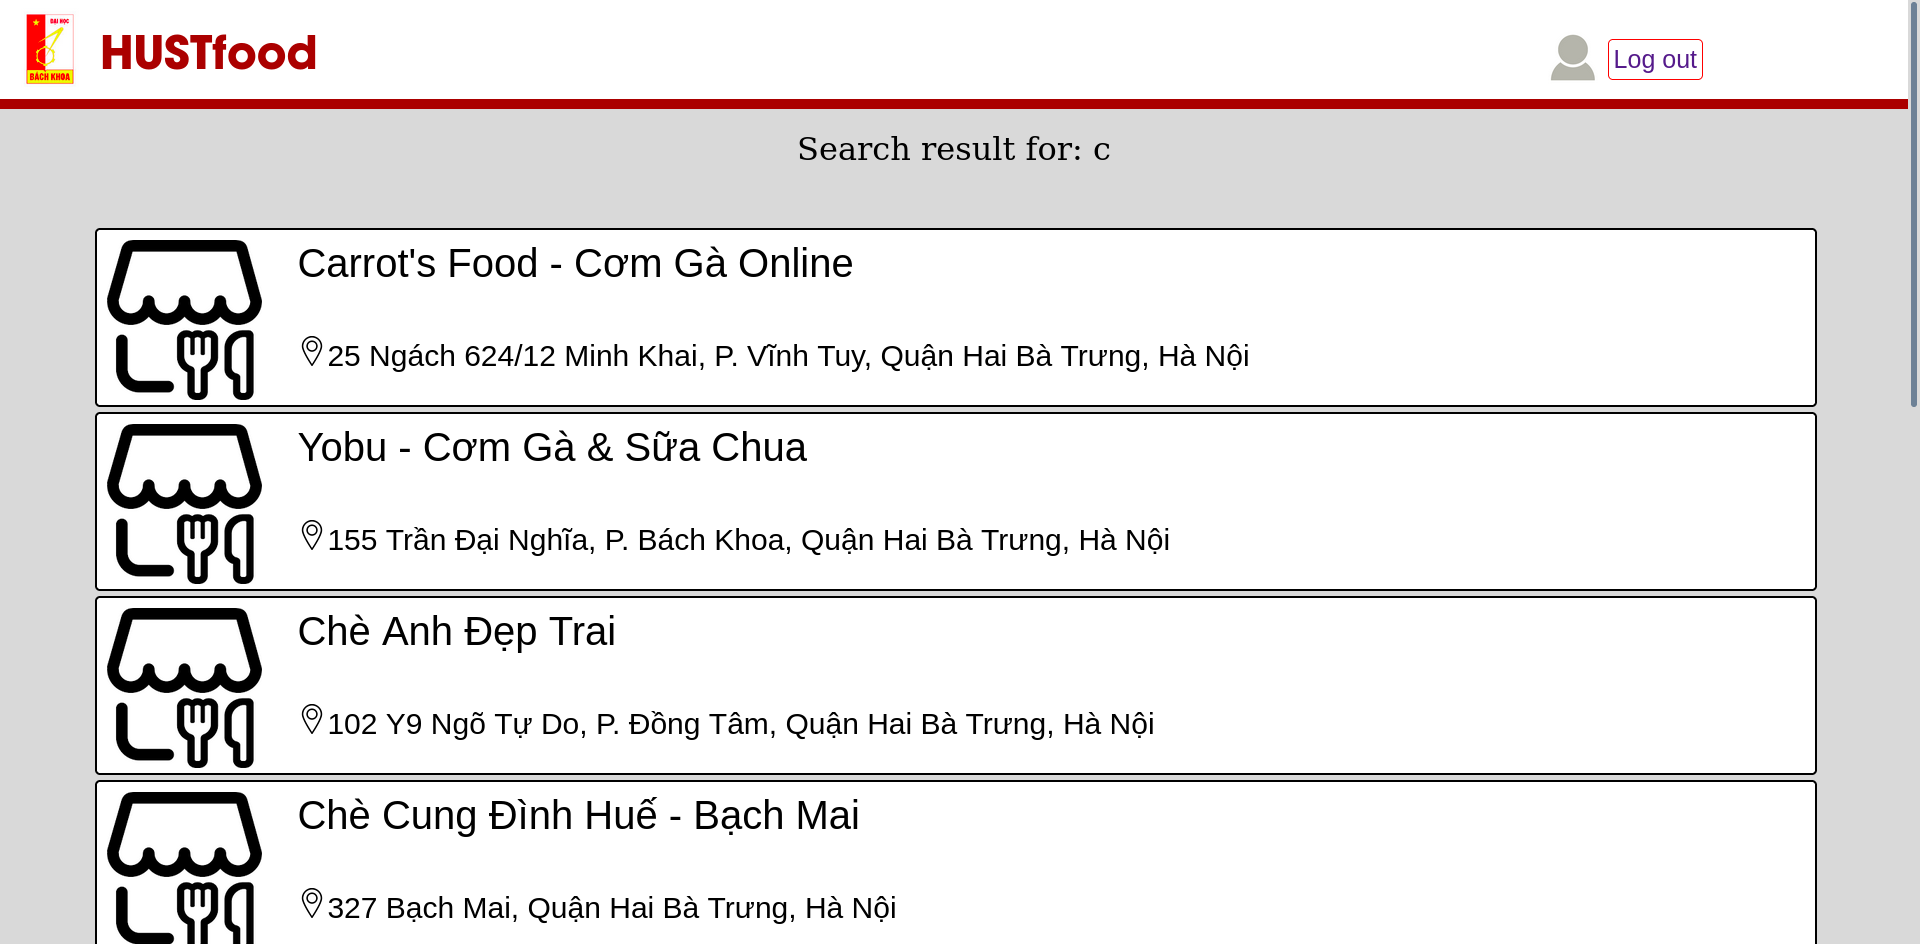
\includegraphics[width=0.9\textwidth]{web-image/timkiem.png}}
			\caption{Giao diện kết quả tìm kiếm}
			\label{fig:ass1}
		\end{figure}
	\end{frame}
	%tìm kiếm bằng cách nào
	\subsection{Menu quán ăn}
	\begin{frame}{Menu quán ăn}
	Hiển thị tất cả các món ăn nhà hàn cung cấp và giá của chúng. Cho phép xem chi tiết món ăn khi chọn "View detail". 
		\begin{figure}[ht!]
			\centerline{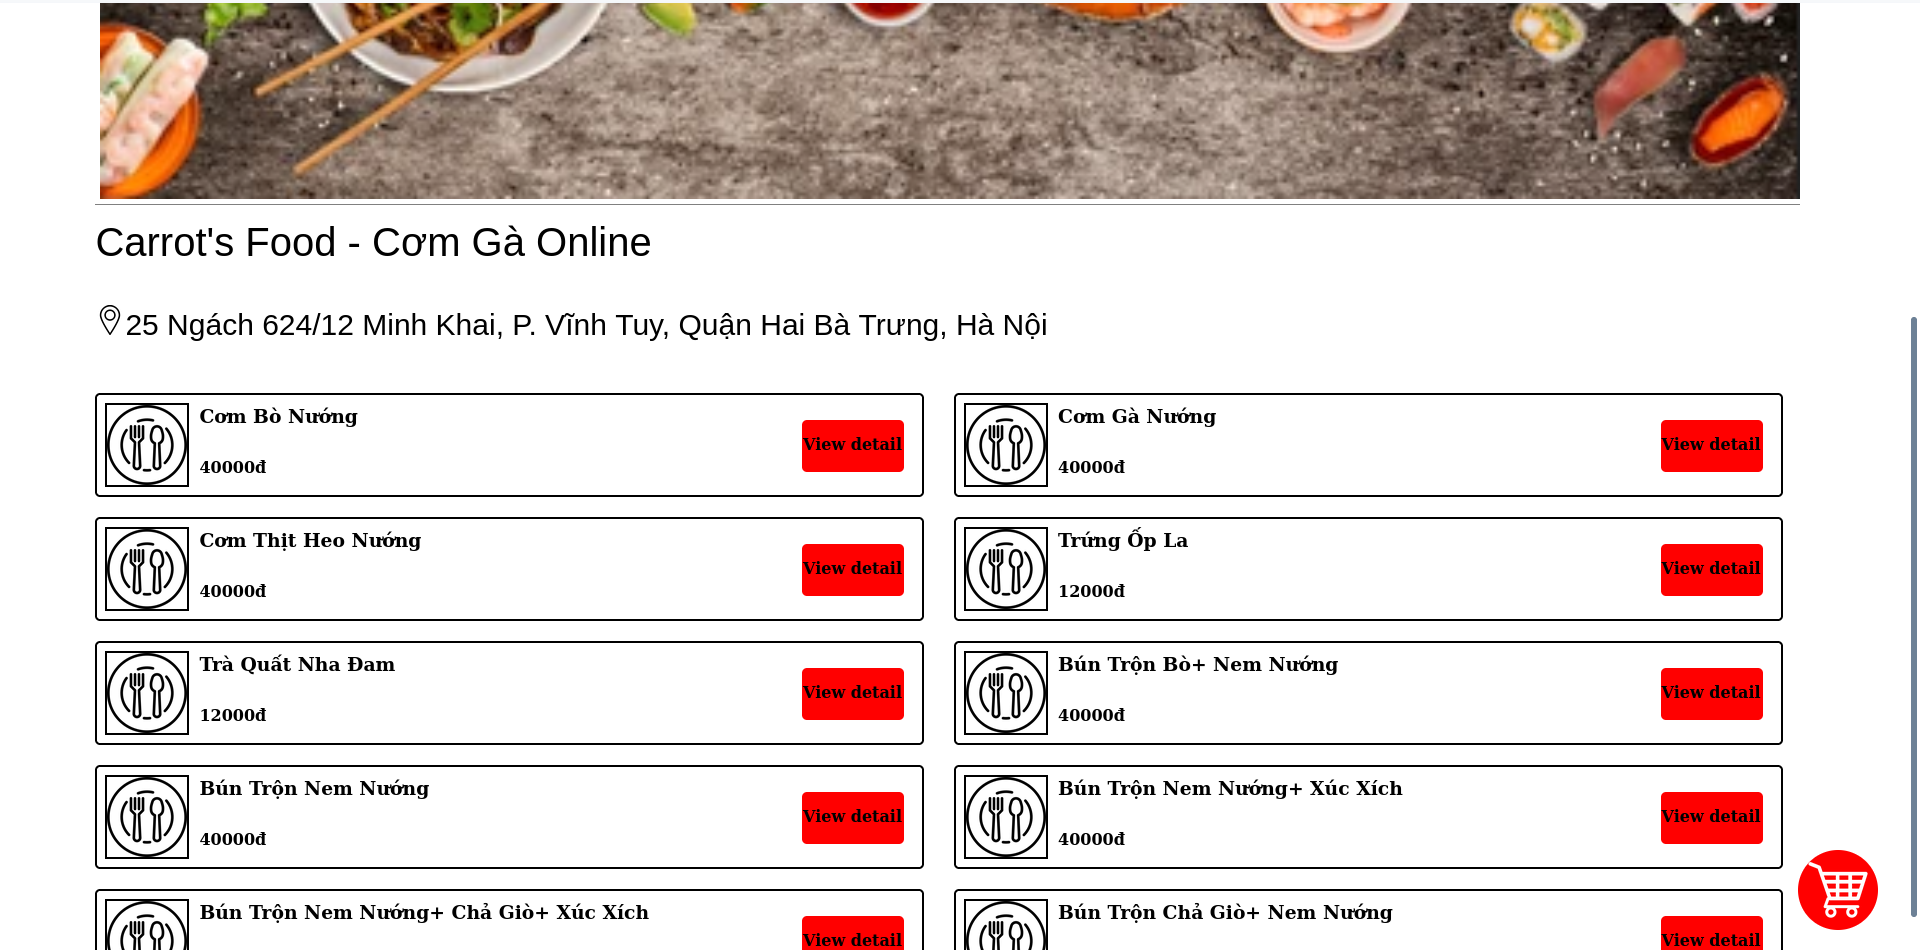
\includegraphics[width=0.9\textwidth]{web-image/nhahang.png}}
			\caption{Các món ăn của nhà hàng}
			\label{fig:ass1}
		\end{figure}
	\end{frame}
	\subsection{Thông tin món ăn}
	\begin{frame}{Thông tin món ăn}
	Cho biết đơn giá của món ăn và cho phép thêm món ăn vào giỏ hàng với số lượng tùy chọn.
		\begin{figure}[ht!]
			\centerline{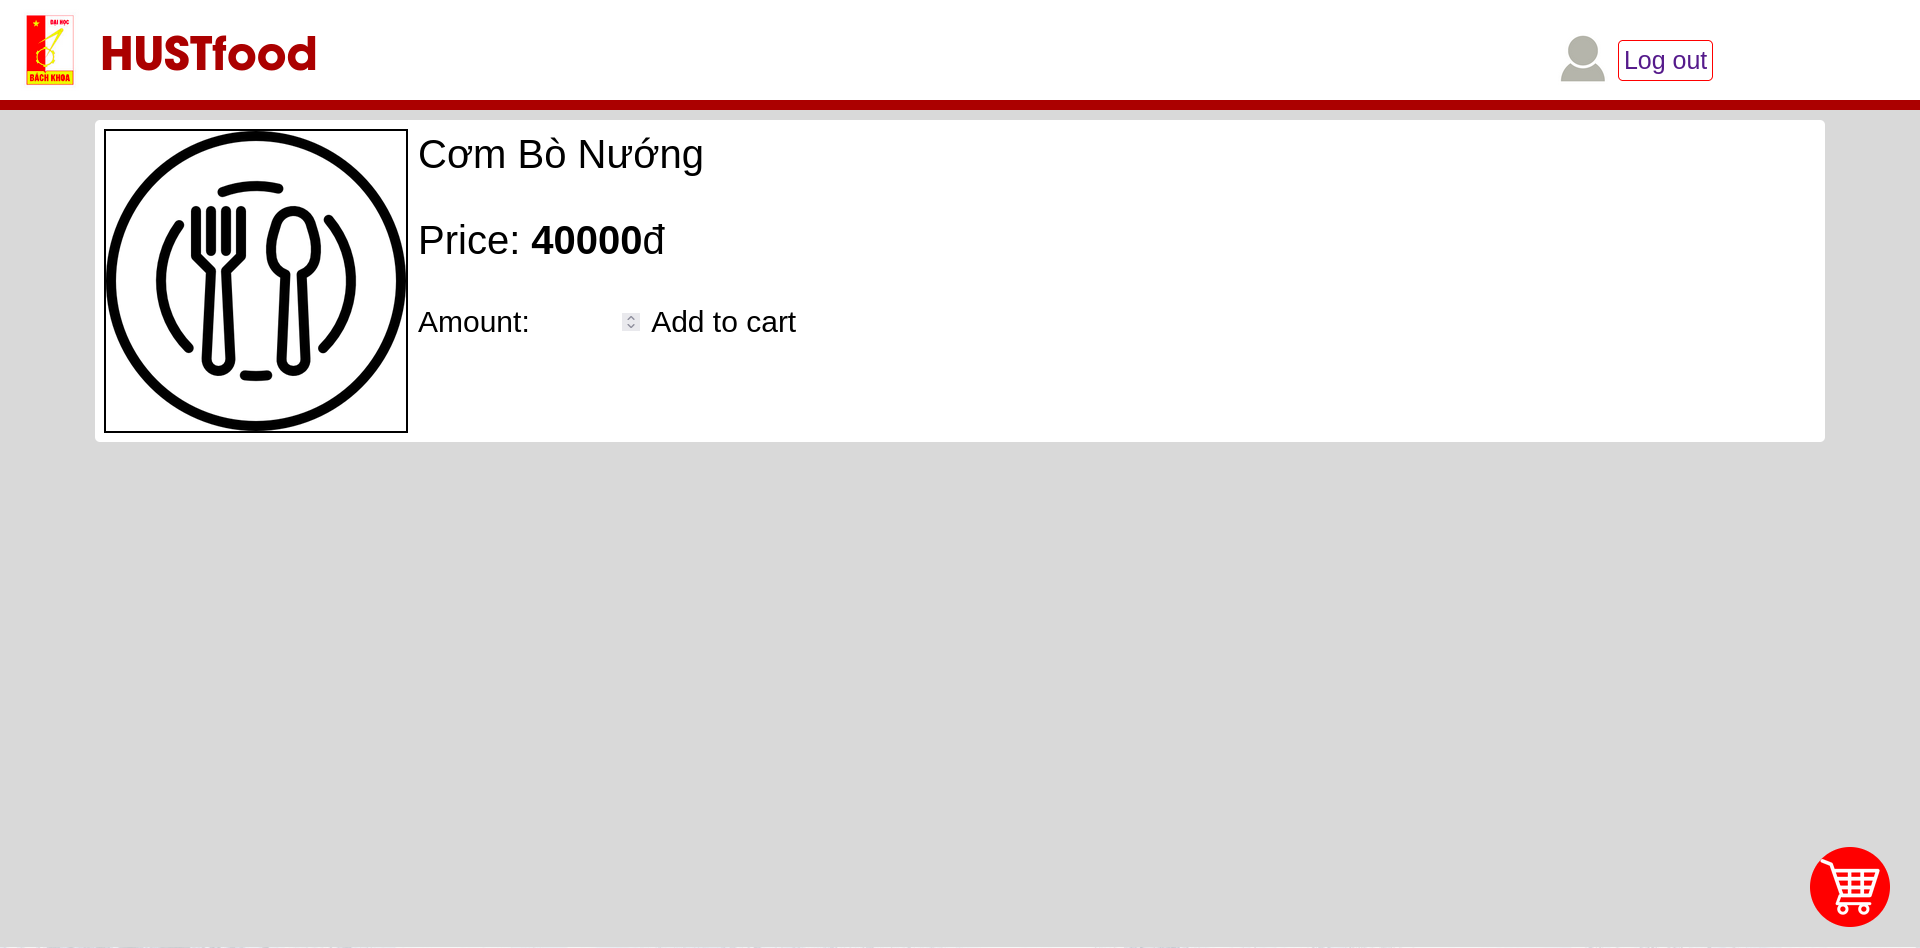
\includegraphics[width=0.9\textwidth]{web-image/Item.png}}
			\caption{Giao diện thông tin món ăn}
			\label{fig:ass1}
		\end{figure}
	\end{frame}
	\subsection{Giỏ hàng}
	\begin{frame}{Giỏ hàng}
	Hiển thị các món đã chọn với đơn giá, số lượng và tổng số tiền phải trả. Cho phép chọn phương thức thanh toán và lựa chọn thanh toán đơn hàng hoặc tiếp tục chọn món.
		\begin{figure}[ht!]
			\centerline{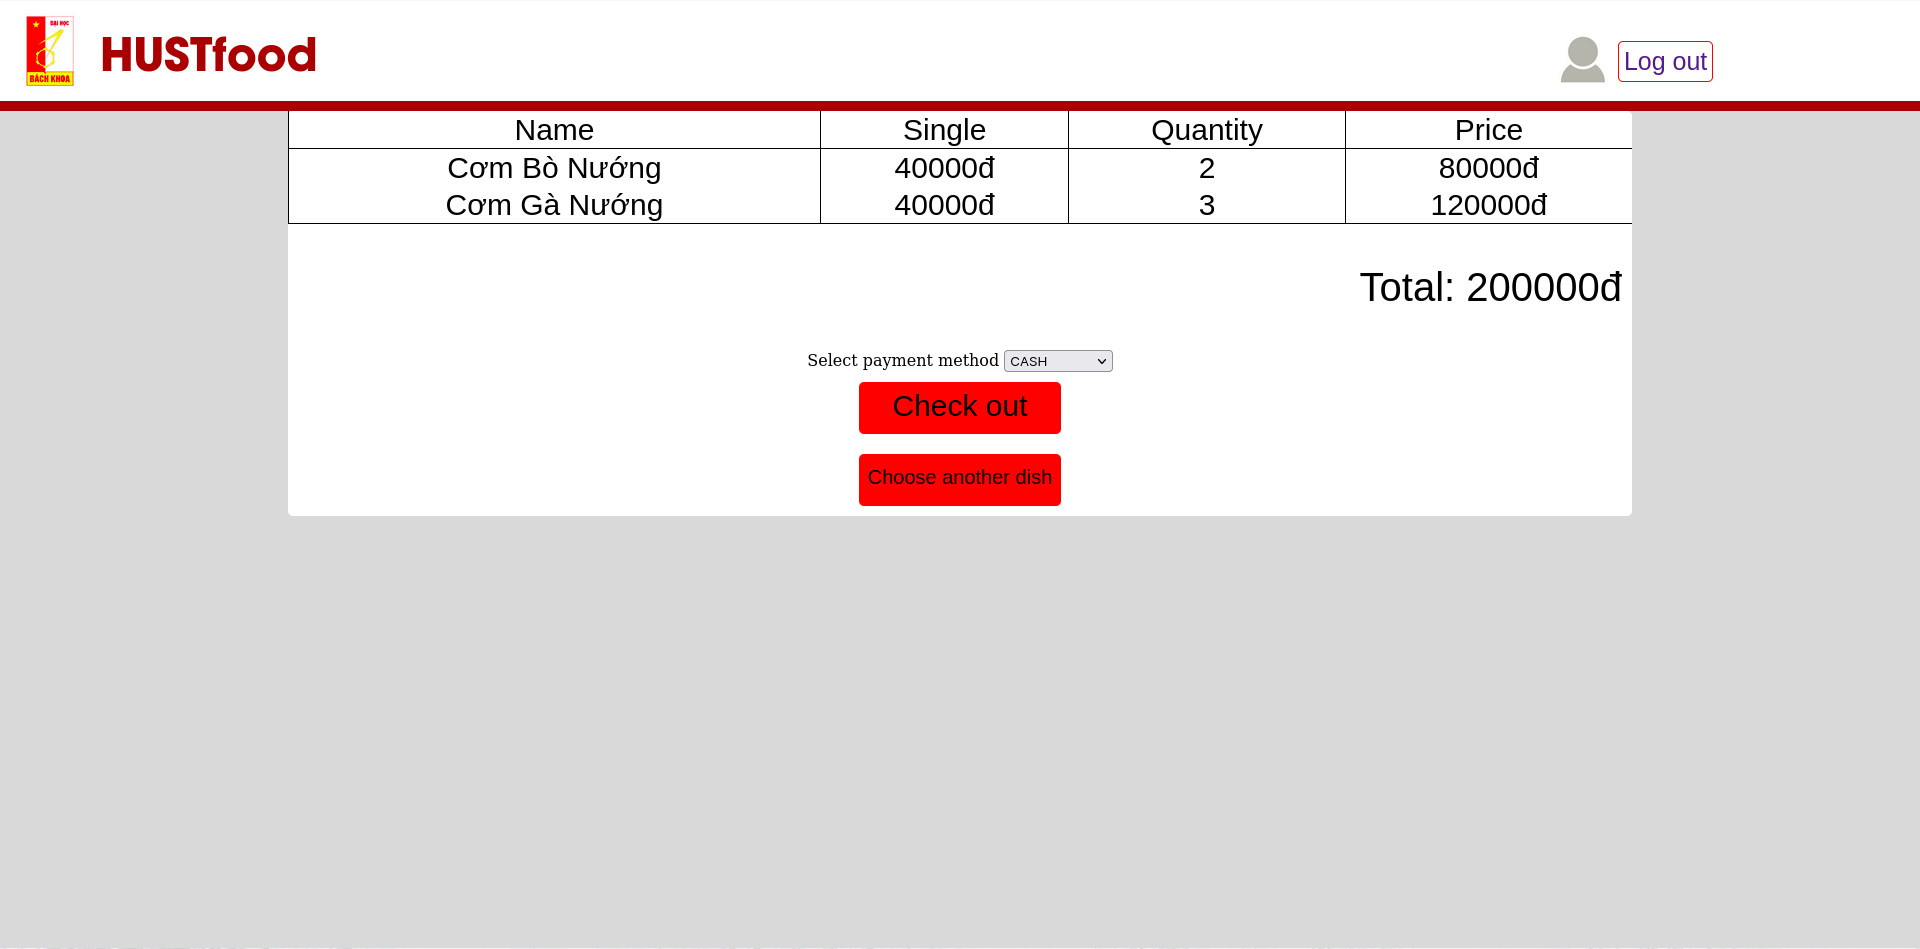
\includegraphics[width=0.9\textwidth]{web-image/giohang.png}}
			\caption{Giao diện giỏ hàng}
			\label{fig:ass1}
		\end{figure}
	\end{frame}
	\begin{frame}[plain, noframenumbering]
		\Huge{\centerline{\textbf{The End}}}
	\end{frame}
\end{document}